\section{Problems}

\noindent {\bf Problem \thesection.\theprob}\stepcounter{prob}

A fan conveys air that's density is $1.2~\frac{\mathrm{kg}}{\mathrm{m^3}}$. 
%The pressure at the suction side is approximately the atmospheric pressure, at the pressure side the pressure is $200~\mathrm{Pa}$ higher. 
The pressure difference between the pressure and suction sides is $200~\mathrm{Pa}$. 
The volumetric flow rate is $Q=0.4~\frac{\mathrm{m^3}}{\mathrm{s}}$, the diameter of the duct at the suction side is $D_1=200~\mathrm{mm}$, and the duct diameter at the pressure side is $D_2=250~\mathrm{mm}$. Find the static and total pressure difference created by the fan! Find the useful power of the fan! (Solution: $\Delta p_{stat} = 102.8~\mathrm{Pa}$, $\Delta p_{tot} = 142.6~\mathrm{Pa}$, $P_u = 57.03~\mathrm{W}$). 


%%%%%%%%%%%%%%%%%%%%%%%%%%%%%%%%%%%%%%%%%%%%%%%%%%%%%%%%%%%%%%%%%%%%

\vspace{1cm}
\noindent {\bf Problem \thesection.\theprob}\stepcounter{prob}

The mean diameter of an axial fan is $D_m = 500~\mathrm{mm}$, the speed of rotation is $n=1450~\frac{1}{\mathrm{min}}$. The inlet blade angle is $\beta_1 = 9.1^\circ$, the blade angle at the outlet is $\beta_2 = 12.3^\circ$, and the axial velocity is $c_{ax} = 6.2~\frac{\mathrm{m}}{\mathrm{s}}$. Find the ideal total pressure difference created by the fan using Euler's turbine equation! What is the actual total pressure difference, if the hydraulic efficiency is $\eta_h=80\%$? Find the static pressure difference! (Solution: $\Delta p_{tot,id} = 433.9~\mathrm{Pa}$, $\Delta p_{tot} = 347.1~\mathrm{Pa}$, $\Delta p_{stat} = 324.1~\mathrm{Pa}$).


%%%%%%%%%%%%%%%%%%%%%%%%%%%%%%%%%%%%%%%%%%%%%%%%%%%%%%%%%%%%%%%%%%%%%%

\vspace{1cm}
\begin{tcolorbox}
\noindent {\bf Problem \thesection.\theprob}\stepcounter{prob}

How does the pressure difference change for the axial CPU fan in Problem 2.2.12, if we install guiding vanes after the fan that eliminate the circumferential velocity component of the flow at the exit? 

(Note that this problem is only a demonstration of the calculation. In reality, CPU fans are never equipped with guiding vanes, because their efficiency is not the most important parameter. A more important parameter of CPU fans is noise.)
%Find the inlet blade angle of the guiding vanes!

Solution:
The calculation of problem 2.2.12:
\begin{itemize}
\item $A_{ring}=\frac{\left(D_o^2-D_i^2\right)\pi}{4}=0.00137\,\mathrm{m^2}$
\item $D_{mean}=\frac{D_o+D_i}{2}=0.03425\,\mathrm{m}$
\item $u_{mean}=u_1=u_2=D_{mean}\pi n=4.913\,\mathrm{\frac{m}{s}}$
\item $c_{ax}=c_{1,ax}=c_{2,ax}=u \tan\beta_1=1.788\,\mathrm{\frac{m}{s}}$
\item $q=\eta_{vol}A_{ring}c_{ax}=0.00184\,\mathrm{\frac{m^3}{s}}$
\item $w_{2u}=\frac{c_{ax}}{\tan\beta_2}=2.131\,\mathrm{\frac{m}{s}}$
\item $\Delta c_u=u-w_{2u}=2.782\,\mathrm{\frac{m}{s}}$
\item $\Delta p_{total,ideal}=\rho u\Delta c_u=17.1\,\mathrm{Pa}$
\item $\Delta p_{total}=\eta_h \Delta p_{total,ideal}=14.5\,\mathrm{Pa}$
\end{itemize}

The guiding vane eliminates the circumferential velocity component, while the axial velocity remains the same because the continuity equation needs to be satisfied. Using all this information, we can use Bernoulli's equation between the inlet and the outlet of the guiding vane:
\begin{align*}
& p_2 + \frac{\rho}{2}c_2^2 = p_2 + \frac{\rho}{2} (c_{ax}^2 + c_{2u}^2) = p_3 + c_3^2 = p_3 + c_{ax}^2. 
\end{align*} 
In the equation above, the index 2 denotes the outlet of the impeller blade, which is the same as the inlet of the guiding vane; the index 3 denotes the outlet of the guiding vane. From this equation, the pressure difference $p_3 - p_2$ can be calculated:
\begin{align*}
& dp = p_3 - p_2 = \frac{\rho}{2}c_{2u}^2 = \frac{1.25}{2}\cdot 2.782^2 = 4.838~\mathrm{Pa}. \\
& \Delta p_{total,vane} = \Delta p_{total} + dp = 19.36~\mathrm{Pa}.
\end{align*}
\end{tcolorbox}
%The inlet angle of the guiding vane 


%%%%%%%%%%%%%%%%%%%%%%%%%%%%%%%%%%%%%%%%%%%%%%%%%%%%%%%%%%%%%%%%%%%%%%

\vspace{1cm}
\noindent {\bf Problem \thesection.\theprob}\stepcounter{prob}

The acoustic power in a bus station is $P_{ac} = 4.3~\mathrm{mW}$. Find the acoustic power level! How does the power level change, if the acoustic power changes to $P_{ac,1} = 2P_{ac}$, $P_{ac,2} = 5P_{ac}$, $P_{ac,3} = 8P_{ac}$, $P_{ac,4} = 0.1P_{ac}$? (Solution: $L_w = 96.33~\mathrm{dB},~L_{w,1} = 99.35~\mathrm{dB},~L_{w,2} = 103.32~\mathrm{dB},~L_{w,3} = 105.37~\mathrm{dB},~L_{w,4} = 86.33~\mathrm{dB}$).


%%%%%%%%%%%%%%%%%%%%%%%%%%%%%%%%%%%%%%%%%%%%%%%%%%%%%%%%%%%%%%%%%%%%%%
% feladatgyujtemeny 11.2
\vspace{1cm}
\noindent {\bf Problem \thesection.\theprob}\stepcounter{prob}

An axial fan, which has no guiding vanes, conveys air at volumetric flow rate $Q=2~\frac{\mathrm{m^3}}{\mathrm{s}}$, density $\rho=1.2~\frac{\mathrm{kg}}{\mathrm{m^3}}$, while the static pressure difference is $p_{st} = 120~\mathrm{Pa}$. Find the total pressure difference, if the  diameter of the pipe is $D=450~\mathrm{mm}$! Find the useful power! Calculate the efficiency, if the power of the motor is $P_{in} = 500~\mathrm{W}$! The speed of the fan is $n=960~\frac{\mathrm{1}}{\mathrm{min}}$. Find the sound power level of the fan, using the formula: $L_W = 97 + 10\cdot \log_{10}(Q\cdot \Delta p_{tot} \cdot (\frac{1}{\eta}-1)) + 32\cdot \log_{10}(\frac{u_2}{a})(\mathrm{dB})$. The sonic speed is $a=340~\frac{\mathrm{m}}{\mathrm{s}}$. Draw the velocity triangles at the tip of the fan! In the calculations, you can ignore the fact that the hub locally increases the velocity, and the leakage losses and the loss due to the circumferential velocity component can be also ignored.

(Solution: $\Delta p_{tot} = 215~\mathrm{Pa}$, $P_u = 430~\mathrm{W}$, $\eta = 0.86$, $L_W = 77.8~\mathrm{dB}$, $u = 22.62~\frac{\mathrm{m}}{\mathrm{s}}$, $c_{ax} = 12.58~\frac{\mathrm{m}}{\mathrm{s}}$, $\Delta c_{u} = 7.92~\frac{\mathrm{m}}{\mathrm{s}}$)

%%%%%%%%%%%%%%%%%%%%%%%%%%%%%%%%%%%%%%%%%%%%%%%%%%%%%%%%%%%%%%%%%%%%%%
% feladatgyujtemeny 11.3
\vspace{1cm}
\noindent {\bf Problem \thesection.\theprob}\stepcounter{prob}

The dryers in a forage dryer facility are spatially separated. The air to the dryers is conveyed by two identical centrifugal fans, that's performance curve is $\Delta p_{fan,tot} = 1200 - 300\Big(\frac{\mathrm{Pa}\cdot\mathrm{s^2}}{\mathrm{m^6}} \Big)Q^2$. The characteristic curve of the dyers is $\Delta p_{dryer,tot} = 900\Big(\frac{\mathrm{Pa}\cdot\mathrm{s^2}}{\mathrm{m^6}}\Big) Q^2$. Find the volumetric flow rate, is one dryer is connected one fan! Find the operating point, if two in parallel connected dryers are supplied by (i) two fans in series connection or (ii) two fans in parellel connection!

(Solution:$Q_1 = 1~\frac{\mathrm{m^3}}{\mathrm{s}}$, $Q_{series} = 1.706~\frac{\mathrm{m^3}}{\mathrm{s}}$, $Q_{parallel} = 2~\frac{\mathrm{m^3}}{\mathrm{s}}$)

%%%%%%%%%%%%%%%%%%%%%%%%%%%%%%%%%%%%%%%%%%%%%%%%%%%%%%%%%%%%%%%%%%%%%%
% feladatgyujtemeny 11.4
\vspace{1cm}
\begin{tcolorbox}
\noindent {\bf Problem \thesection.\theprob}\stepcounter{prob}

The "snow cannon" of a ski slope is an axial fan, that accelerates air that's density is $\rho = 1.32~\frac{\mathrm{kg}}{\mathrm{m^3}}$ to velocity $c=30~\frac{\mathrm{m}}{\mathrm{s}}$. Following the impellers, a mass flow rate of $\dot{m}=4~\frac{\mathrm{kg}}{\mathrm{s}}$ water is sprayed into the air, and the water is accelerated to the speed of the air. Find the impulse change of the water! Find the pressure required to accelerate the water, if the cross-section of the of the fan after the impellers is $A=0.2~\mathrm{m^2}$. Find the static and total pressure difference, if the air-water mixture exits directly to the open after the fan! Sketch the static and total pressure along a streamline!

\begin{itemize}
%
\item The watr needs to be accelerated from 0 to 30 m/s; the impulsa change is $\Delta I = \dot{m}_w c=120~\frac{\mathrm{kg m}}{\mathrm{s^2}}$.
%
\item This impulse change is coeverd by the pressure difference of the pump: $A\Delta p=\Delta I$, hence $\Delta p=600$Pa.
%
\item After the water injection, the average density of the water-air mixture is $\rho_m=\frac{Q_{air}\rho_{air}+Q_w\rho_w}{Q_{air}+Q_{water}}=\frac{30 m/s\times 0.2m^2+4kg/s}{6m^3/s+0.004 m^3/s}$, which is the weighted average of the densities, wieghted by the mass flow rates. We also have $Q_{air}=30 m/s\times 0.2m^2=6m^3/s$ and $Q_w=4kg/s/1000 kg/m^3=0.004m^3/s$.
%
 \item The dynamic pressure of the mixture is $894~\mathrm{Pa}$, see Figure \ref{fig:snow_cannon}.
\end{itemize}
\end{tcolorbox}

\begin{figure}[!ht]
\centering
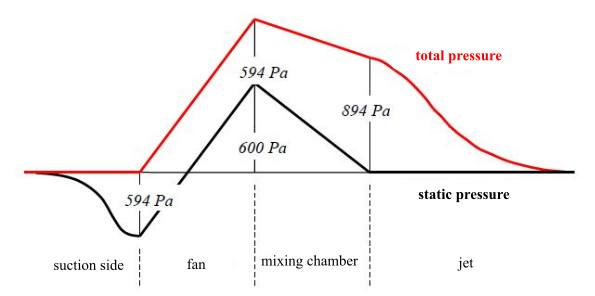
\includegraphics[width = 0.5\textwidth]{Problem_solving/figs/snow-cannon.png}
\caption{\label{fig:snow_cannon} Pressure distribution in the "snow cannon".}
\end{figure}

%%%%%%%%%%%%%%%%%%%%%%%%%%%%%%%%%%%%%%%%%%%%%%%%%%%%%%%%%%%%%%%%%%%%%%
% feladatgyujtemeny 11.7
\vspace{1cm}
\noindent {\bf Problem \thesection.\theprob}\stepcounter{prob}

\begin{wrapfigure}{R}{0.4\textwidth}
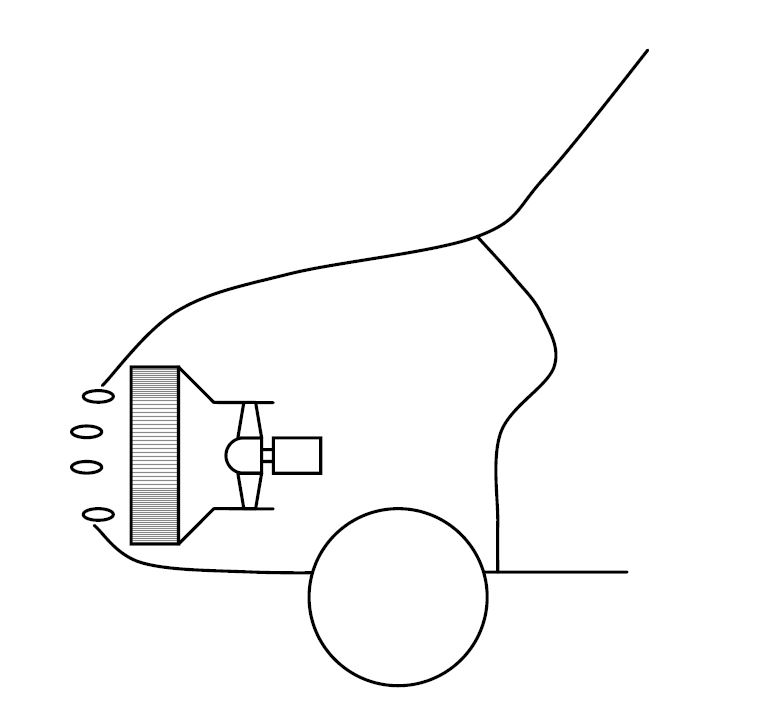
\includegraphics[width=0.4\textwidth]{Problem_solving/figs/car-engine-cooler.JPG}
\end{wrapfigure}

The nominal area of the radiator of a car engine cooler is $A=0.12~\mathrm{m^2}$, and it's loss coefficient is $\zeta = 1.2$. The performance curve of the cooling fan is $\Delta p_{tot} = 147 (\mathrm{Pa}) - 300\cdot \Big(\frac{\mathrm{Pa}\cdot\mathrm{s^2}}{\mathrm{m^6}} \Big)(Q-0.3)^2$. The fan conveys the hot air with density $\rho=1.1~\frac{\mathrm{kg}}{\mathrm{m^3}}$ from it's suction side through the radiator. The outer diameter of the fan is $D_o = 310~\mathrm{mm}$, and the hub diameter is $D_i = 140~\mathrm{mm}$. The air, after it leaves the fan, arrives to the engine space and slows down, while it's pressure reaches the pressure of the ambient air. 

Write down Bernoulli's equation for a stading car, between the far-field point in front of the radiator and the suctions side of the fan, and an other Bernoulli-equation between the pressure side of the fan and the engine space. Using these equations and the performance curve of the fan, find the volumetric flow rate! Sketch the static, dynamic and total pressure along a streamline, between the far field point - suction side and the pressure-side - engine space!

(Solution: $Q=0.7036~\frac{\mathrm{m^3}}{\mathrm{s}}$)

%%%%%%%%%%%%%%%%%%%%%%%%%%%%%%%%%%%%%%%%%%%%%%%%%%%%%%%%%%%%%%%%%%%%%%
% feladatgyujtemeny 11.5
\vspace{1cm}
\noindent {\bf Problem \thesection.\theprob}\stepcounter{prob}

Find the relative pressure needed to support an inflatable tennis court tent, id the are if the tent is $22\times 40~\mathrm{m^2}$, and the mass of the tent is $m=3000~\mathrm{kg}$. How long does it take to set up such an inflatable tent, if the performance curve of the fan we use is $\Delta p_{tot} = 70~\mathrm{Pa} - 42\cdot \Big(\frac{\mathrm{Pa}\cdot\mathrm{s^2}}{\mathrm{m^6}} \Big)Q^2$ and the average height of the tent is 5 m? The density of the air is $\rho = 1.3~\frac{\mathrm{kg}}{\mathrm{m^3}}$, the cross-section of the fan at the pressure side is $A=0.2~\mathrm{m^2}$, and the fan conveys the air between two open spaces! Find the stationary leakage flow rate from the tent, if the area of the holes on the tent (which ensure a cross flow through the tent to provide fresh air) is $A_l = 0.05~\mathrm{m^2}$! Find the relative pressure in the tent!

(Solution: $\Delta p = 33.4~\mathrm{Pa}$, $t=1.54~\mathrm{h}$, $v=0.469~\frac{\mathrm{m^3}}{\mathrm{s}}$, $\Delta p_{stat} = 57~\mathrm{Pa}$)



